%!TEX root = ../crimson_throne_book_main.tex
% 2015-03-14
Before the companions lies what looks like the entry hall to the secret hide-out underneath the Hospice of the Blessed Maiden. The hall sits empty and seems recently redecorated with murals of skeletons feasting among the dead and diseased citizens of Korvosa. The paintings are crudely done and have already been damaged by water seepage from the surrounding rocks. Simple wooden doors lead in every direction, each bearing a painted scythe-wielding skeleton.\\

Puk and Balian sneak in and listen at the doors. They only pick up something at the one on the right-hand side: people snoring inside! Fantastic! So they still have the element of surprise on their side. The urban ranger and the rogue quietly open the door and find four of the queen's physicians asleep in a small storage room. They waste no time and murder the men in their sleep. Quint is content to learn that his {\itshape principled} friend Sjo has no qualms about these merciless assassination tactics, after all, the physicians' guilt has been clearly established. This is swift and clean justice! The companions now try the left door in the entry hall, which leads to a cloakroom. Two big wardrobes hold several dark leather robes, high boots, wide-brimmed hats and beaked plague masks. Sjo also discovers some {\itshape potions of cure moderate wounds} and a bag with 23 black onyx gems, worth 50 GP each, stuck away behind the robes. There is another door in this room which again reveals the sound of people sleeping on the other side. Quint, who is still wearing the avian mask and leather coat as a disguise, walks in first to find a room filled with cots: there are no less than ten physicians resting in here. As Balian and Puk sneak inside to quietly end these bastards' lives, one of the sleepers stirs and sits up. Quint walks over and tries to set his mind at ease with some casual conversation while his friends slip into position to strike the man down in his bed. The plan works, but the noise seems to have awoken another doctor. Again the companions act fast and kill him before he can raise the alarm. The rest of the sleeping doctors are put to the sword as well. The companions continue their exploration by returning to the central axis of the hide-out. They discover a\hyperref[fig:Bacchanal-of-Urgathoa-beneath-the-Hospice-520054146]{ chamber with a dozen skeletons lining the walls } . Their bony fingers claw in the air and the empty sockets in their skulls stare at the intruders with nightmarish determination. Sjo immediately reaches for his mace, but then he sees that the bones do not move. It seems like some twisted mind set them on display here in a  {\itshape tableau mort} , to remind all the living that they will one day die and their remains might be called upon to serve the Pallid Princess. Urgathoans certainly have a weird concept of art, no wonder they have to hide it under the ground. A heavy, metal door leads deeper into the complex, probably to the temple itself, but the companions leave it for now, deciding to veer off to the right first because they hear voices coming from that side. \\

\begin{figure}[h]
	\centering
	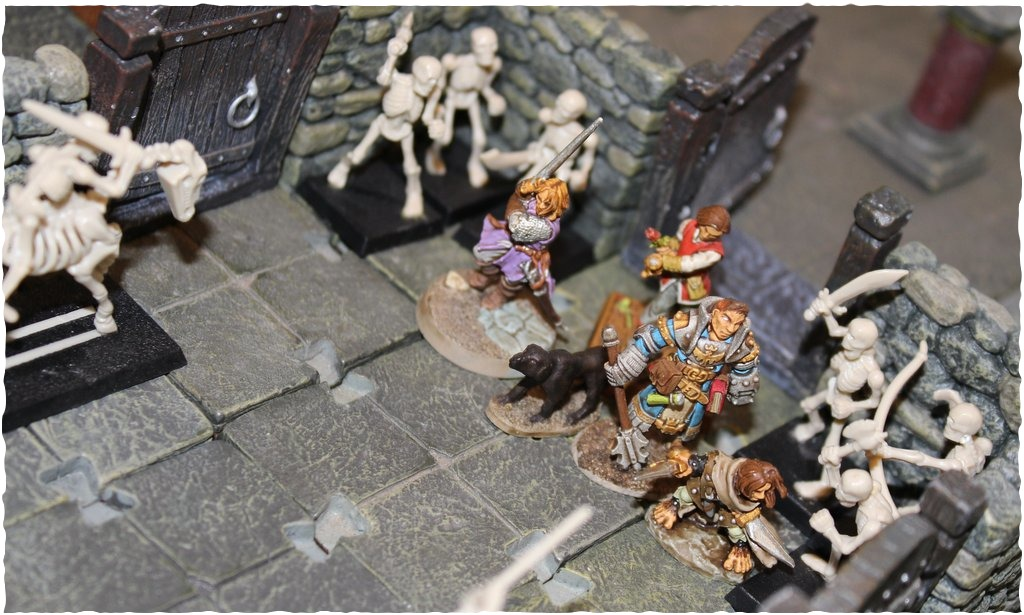
\includegraphics[width=0.4\textwidth]{images/Bacchanal-of-Urgathoa-beneath-the-Hospice-520054146_mod.jpg}
	\caption{Bacchanal of Urgathoa beneath the Hospice}
	\label{fig:Bacchanal-of-Urgathoa-beneath-the-Hospice-520054146}
\end{figure}

Balian picks up an agitated voice through the door. "I tell you again, I'm sorry for disturbing your rest, but there were some fierce-looking guys snooping around upstairs. I know you want to be informed of anything suspicious happening; they were talking about about investigating this place before they suddenly made off, spilling some sorry excuse of having made a mistake. I didn't trust them one bit, but that Gray Maiden officer seemed to believe them and let them go. I discussed it with Sordek upstairs and we finally decided it best to inform you. Better to be safe than sorry, right?"\\

Quint decides to go in first again, making use of his disguise. Swinging open the door he walks into another bedroom with six people, all awake and fully dressed: doctor Saulus, a masked physician, two cultists in a breastplate carrying a scythe, a pale and skinny man, with a blotchy and scarred face, and a dark-haired woman. Quint immediately recognizes the gaunt individual as Rolth, the necromancer, the villain they have been trying to track down for ages. The woman in his company must be the lady who took away all those girls from Gaedran Lamm; the girls they discovered later in the mass grave underneath Lost End, where they had been used as guinea pigs for the plague. The bard still feels sick thinking about it. Still, the black-haired lady looks quite young herself, certainly no older than sixteen or seventeen. In fact, she looks familiar as well ... By the gods, could it be? Is Rolth's black-haired accomplice Balian's sister Alika? Quint tries to swallow down the shock that clumps his throat and tries to catch his bearings as Saulus addresses him: "So, any news from upstairs? Did you see those men again that Geoff here told us about?"\\

"Uhmm, no sir, all's quiet, nothing to report", Quint replies.\\

"Well, we might as well check it out, we're up anyway", Saulus responds as he signals the two cultists to lead the way. While Quint slips deeper into the room to the woman's side, the first cultist walks out of the room, only to be surprised by Balian and Puk, who promptly cut him down. Geoff, the physician who came down to warn Saulus, quickly quaffs a vial and peeks around the corner to see who just killed his cultist buddy. "You see, I told you, it's them, it's them!" he cries.\\

Quint sticks to his role and grabs the lady's arm: "By the gods, intruders! Do you have a weapon for me, {\itshape Alika} ?" In spite of his desire to see it otherwise, the black-haired woman responds to the name  {\itshape Alika} . "Here, take one of my daggers." Balian, who rushes in with Puk to finish the other cultist, picks up the name as well, realizing that he is now facing his sister. He immediately tries to reason with her: "Alika, it's me, Balian, your brother. We've come to free you!"\\

"Huh, my brother to the rescue? After five years? You're nothing but a coward and traitor, and a fool! I have found my true purpose in the service of Urgathoa! Now face her and my wrath!"\\

Meanwhile Saulus and Rolth retreat to the far end of the room and cast defensive spells, as Sjo appears in the door opening and throws his new spell on them, {\itshape fireball} ! Spyder also springs into the chamber, but when he recognizes Alika's scent, \hyperref[fig:Spyder-recognizes-Balian-s-sister-Alika-520054718]{ he starts wagging his tail } . The masked physician pulls out another vial and flings it at Balian: it explodes in a burst of flames. Quint uses his disguise one final time in this combat, to take position at Rolth's side. Then the bard pulls out his sword and hacks away at the necromancer. His blade hits the skin as if it was stone. Darn, he just cast  {\itshape stoneskin} ! Doctor Saulus mutters the words of another spell, trying to  {\itshape slow} Balian, Puk, Spyder and Sjo, but the magic only takes on the dog and the halfling. Alika also moves over and viciously cuts at the slowed rogue, proving to have similar skills in combat with her sneak attack. Rolth realizes the threat the 'physician' at his side poses and steps back, flinging two  {\itshape scorching rays} at the disguised bard. Now it is Quint's turn to smile, because he has an effective magical defense of his own: his ring of fire resistance absorbs the burning damage. Sjo charges to the bard's side and engages Saulus: his heavy mace hits the doctor hard! Balian's greatsword swings even harder on the physician who tries to escape his reach to do another spell, but the ranger  {\itshape steps up} and kills him with one clean stroke. Next he joins his friends in the corner to fight the two powerful mages. His hatred guides his blade at the necromancer, but his anger clouds his combat savvy and he misses the foul caster. Doctor Saulus clearly feels outmatched and tries to swing the balance in his favor by casting  {\itshape improved invisibility} on himself. Sjo and Quint hear him running off and chase after him. Sjo throws a sheet of fire in front of him and the flames of his  {\itshape burning hands} reveal the shape of Saulus. Quint snatches some  {\itshape dust of appearance} from his pocket and blows it in the same direction, breaking the doctor's concealing magic. Still, doctor 'Devils' proves worthy of his nickname when he steps back and calls down the fires of hell! A mighty fireball turns the room into an inferno, but when the licking flames burn out, only Puk and Alika have been badly hurt. Quint and Sjo dodge most of the blaze and their protection from fire wards them from most of the remaining damage. \\

\begin{figure}[h]
	\centering
	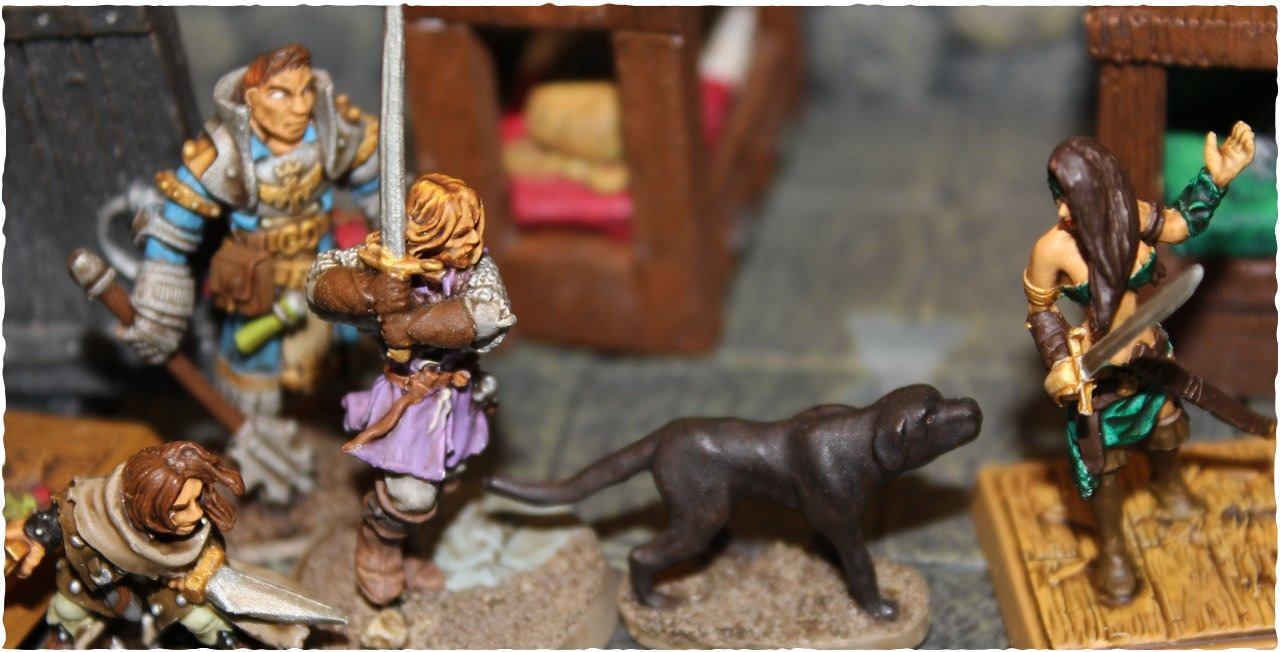
\includegraphics[width=0.4\textwidth]{images/Spyder-recognizes-Balian-s-sister-Alika-520054718_mod.jpg}
	\caption{Spyder recognizes Balian's sister Alika}
	\label{fig:Spyder-recognizes-Balian-s-sister-Alika-520054718}
\end{figure}

The odds are now clearly in favor of the companions: Balian controls his rage and hits down Rolth with the flat side of his blade. Quint and Sjo mock Saulus's feeble attempts at hurting them and cut off his escape route? With Balian's help they knock out the doctor as well.\\

Now only Alika remains. Sjo freezes her in place with a {\itshape hold person} , giving Balian the chance to disarm and bind her before she can move again. So, how does this work? How do you talk to your sister after she has tried to kill you? Especially when you're out of practice with the concepts of brotherly love as Balian is ... 